\chapter{How was the project created?}\label{ch:B}

\section{Project UI}
Stack: postgresql, Django, python, Django ORM. First we structured the DDL diagram for the project database, after that we connected it with django and used the orm system. Most of the logic is the CRUD system. Also there is integration with github api in python where we can reference to their api to send or get some information from user’s githubStack: postgresql, Django, python, Django ORM. First we structured the DDL diagram for the project database, after that we connected it with django and used the orm system. Most of the logic is the CRUD system. Also there is integration with github api in python where we can reference to their api to send or get some information from user’s github %Поменять!!!%
\section{Project Front}
Used mui/material design library for beautiful UI and components respectively. Mui library only used with React js library by Facebook. With React there was used a lot of technologies like Formik, Yup, Lodash etc.
Created centralized components. Example \ref{fig:dgrm}:
\begin{figure}[ht]
    \centering
    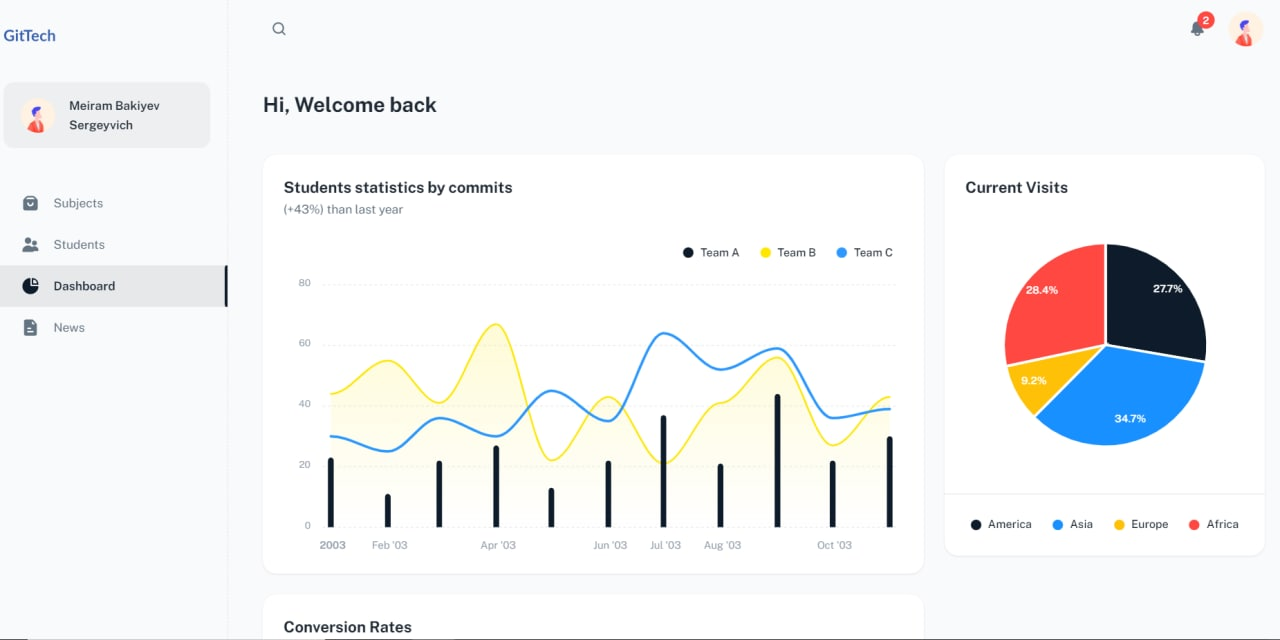
\includegraphics[scale=0.5]{diagramsfnt.jpg}
    \caption{Diagram}
    \label{fig:dgrm}
\end{figure}
Added charts for analytic results, charts like Pie, line. Example \ref{fig:sbj}:
\begin{figure}[ht]
    \centering
    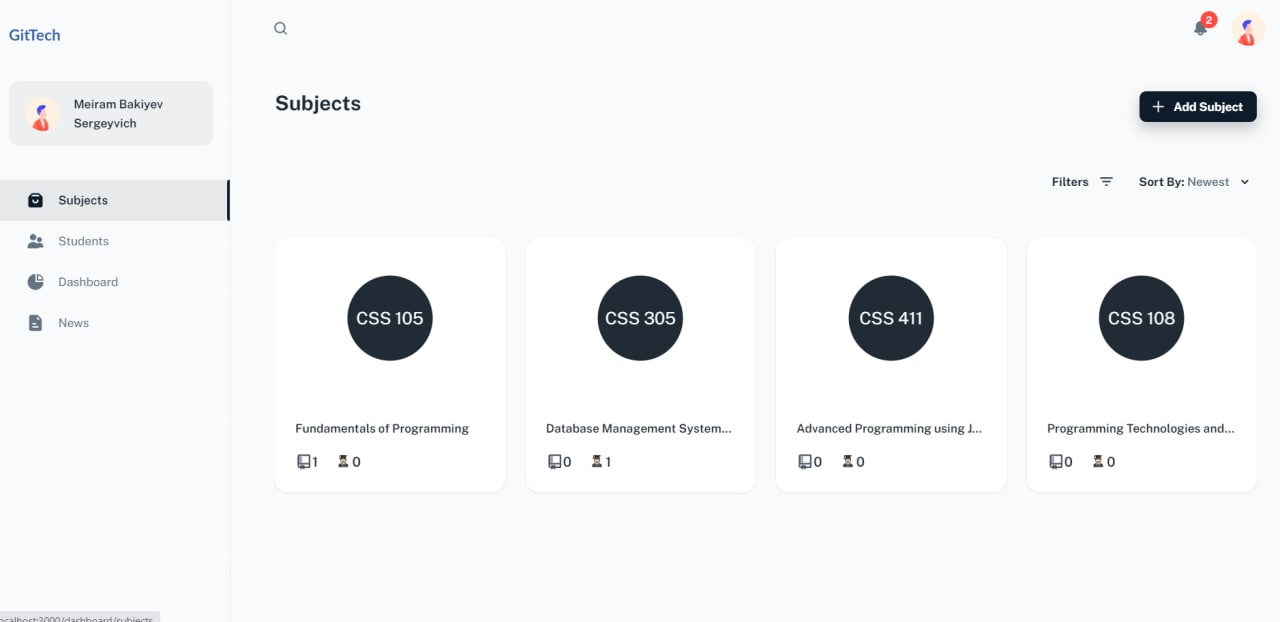
\includegraphics[scale=0.5]{subjectsfnt.jpg}
    \caption{Item selection}
    \label{fig:sbj}
\end{figure}

\section{Project back}
Stack: postgresql, Django, python, Django ORM. First we structured the DDL diagram for the project database, after that we connected it with django and used the orm system. Most of the logic is the CRUD system. Also there is integration with github api in python where we can reference to their api to send or get some information from user’s github